\phantomsection
\section*{PHỤ LỤC. ẢNH KIỂM THỬ BẢO MẬT}
\addcontentsline{toc}{section}{PHỤ LỤC. ẢNH KIỂM THỬ BẢO MẬT}
\label{sec:anh-sec}

Ba ảnh bổ trợ làm rõ cấu hình quyền, kết quả kiểm tra bản ghi trước và sau phép thử B1, và định nghĩa VIEW dùng trong B2.

\begin{figure}[H]
    \centering
    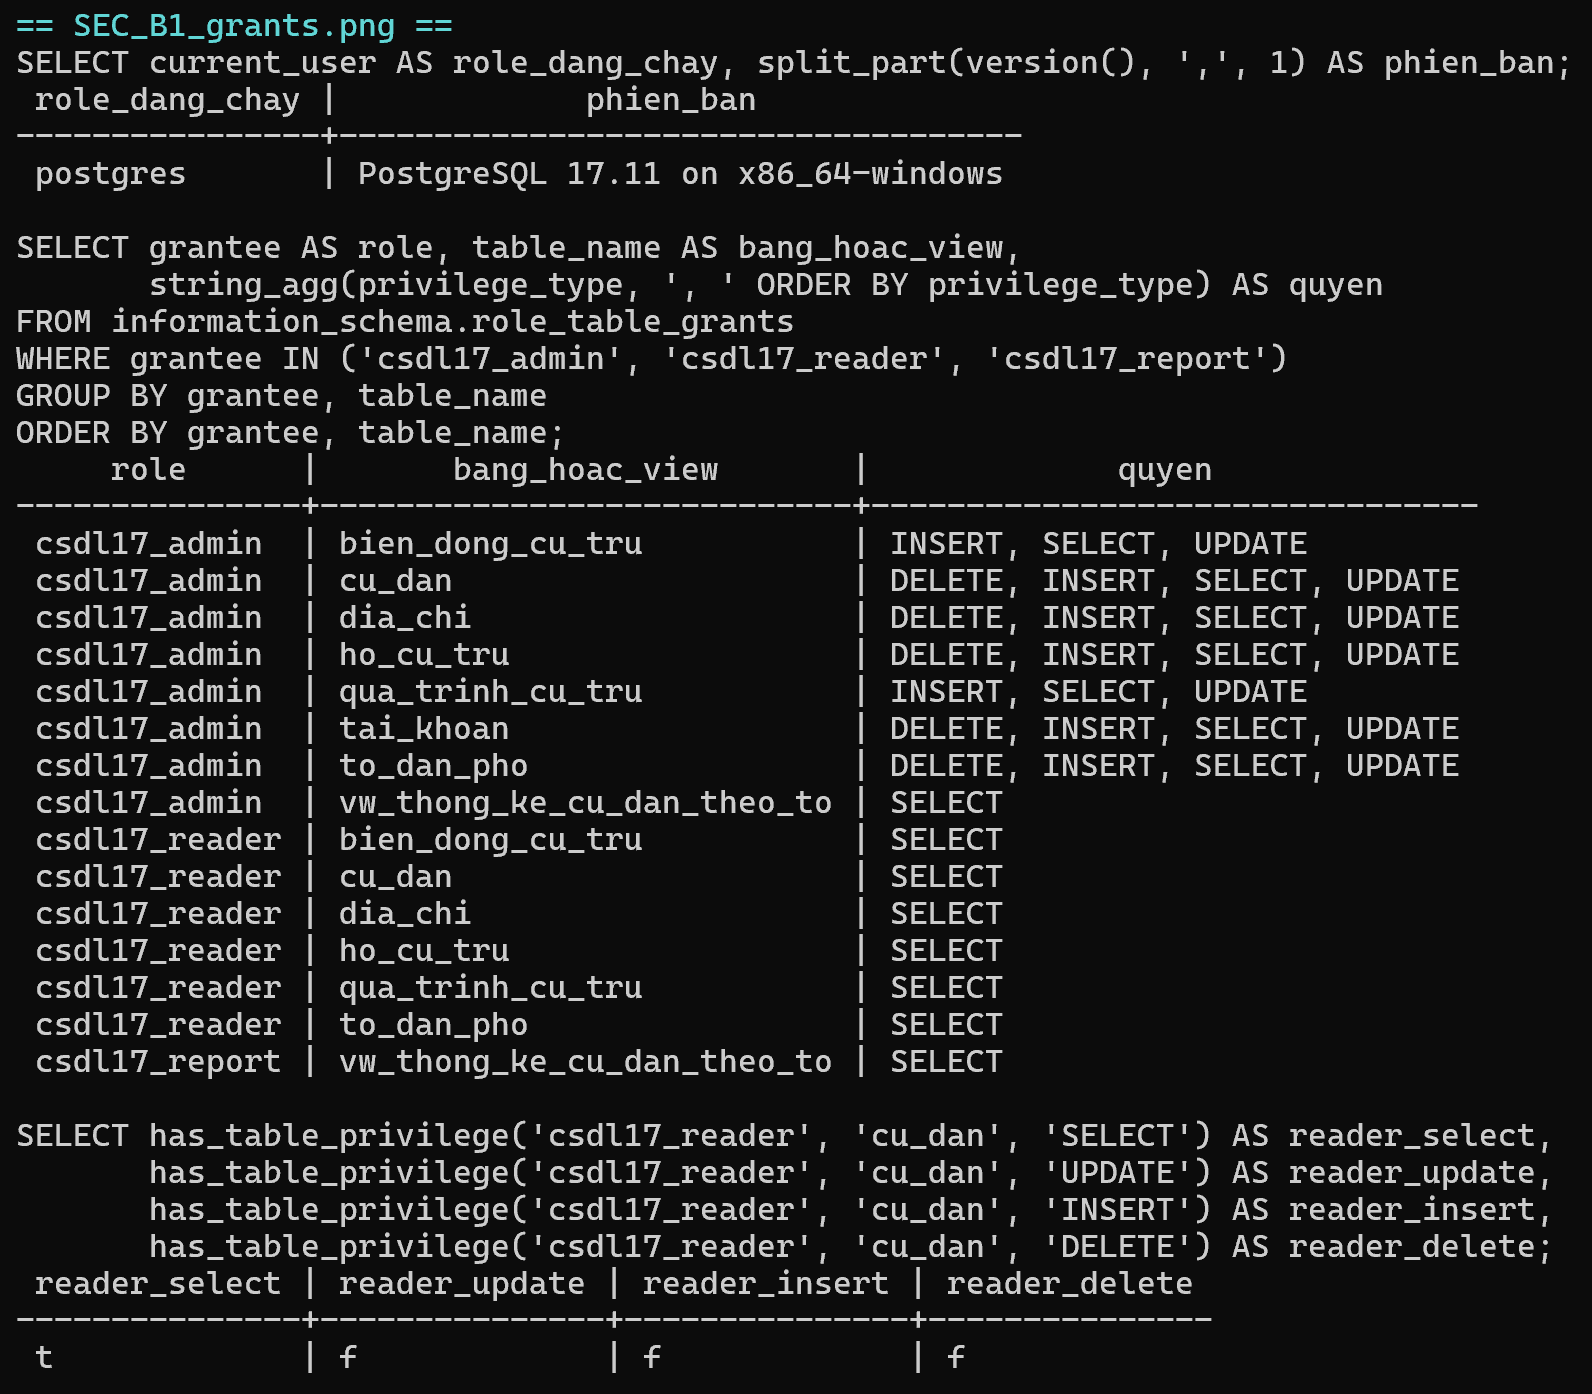
\includegraphics[width=\linewidth,height=.76\textheight,keepaspectratio]{image/security/SEC_B1_grants.png}
    \caption{B1 --- Quyền của ba role trên các bảng và VIEW}
\end{figure}
\clearpage

\begin{figure}[H]
    \centering
    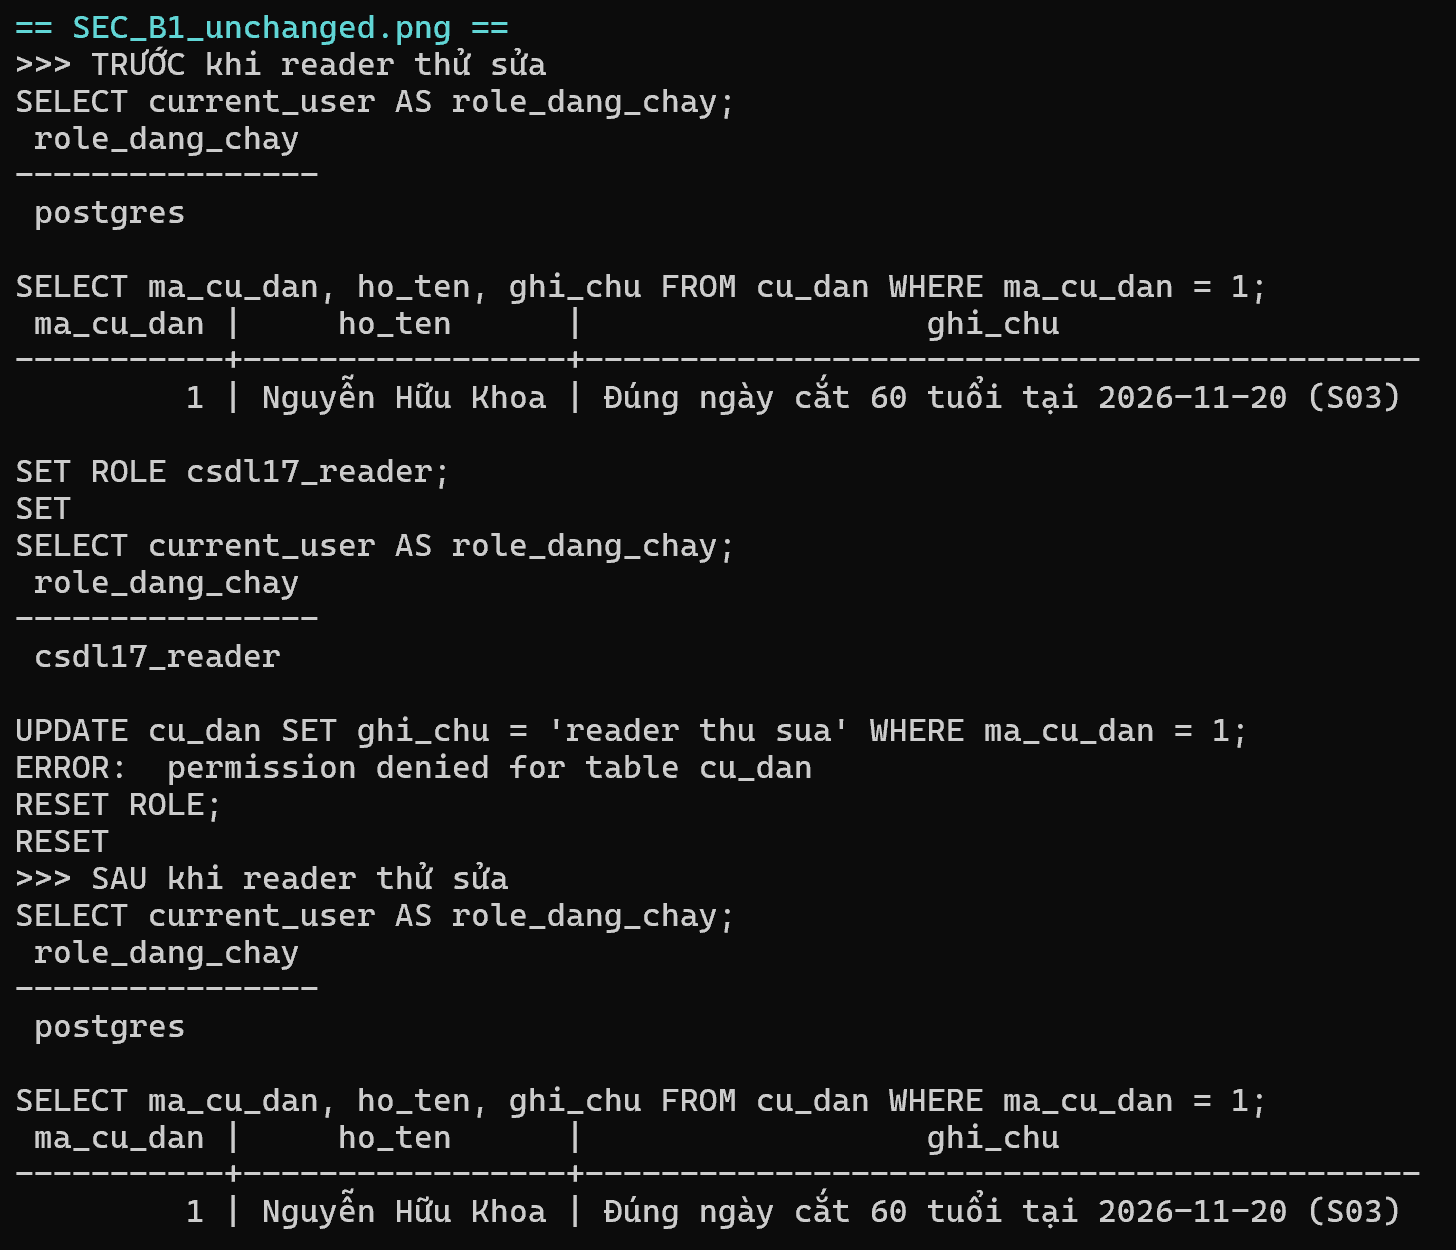
\includegraphics[width=\linewidth,height=.76\textheight,keepaspectratio]{image/security/SEC_B1_unchanged.png}
    \caption{B1 --- Giá trị của bản ghi kiểm tra trước và sau phép thử}
\end{figure}
\clearpage

\begin{figure}[H]
    \centering
    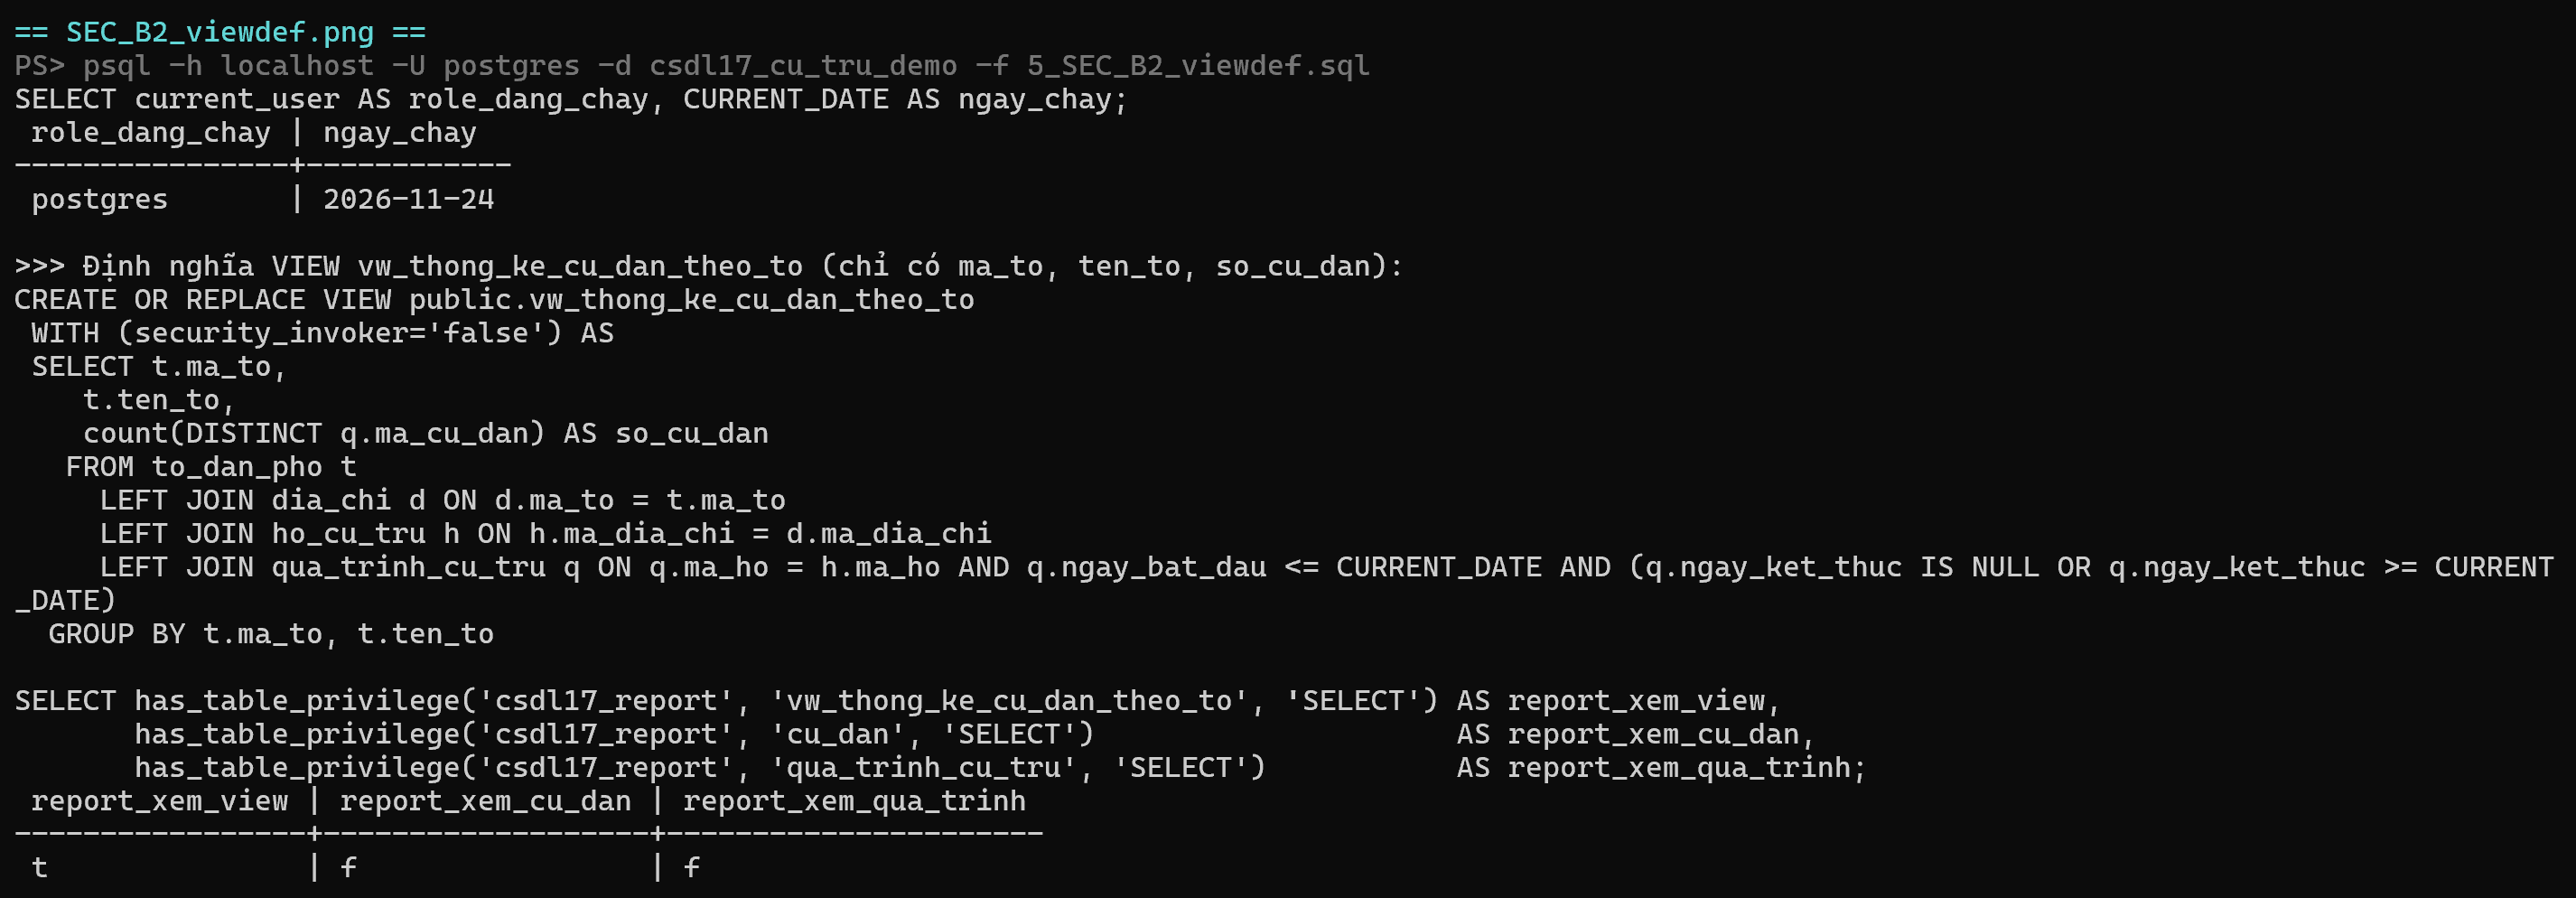
\includegraphics[width=\linewidth]{image/security/SEC_B2_viewdef.png}
    \caption{B2 --- Định nghĩa VIEW trong cơ sở dữ liệu demo và kết quả kiểm tra quyền}
\end{figure}

Ảnh trên được chụp từ bản VIEW thử nghiệm trước đó, dùng \texttt{CURRENT\_DATE} và chạy ngày 24/11/2026. Bản chính thức trong \texttt{sql/05\_security.sql} và ở Chương 6 cố định ngày 20/11/2026. Nhóm đã đếm lại theo cả hai ngày: số cư dân của tám tổ trùng khớp (34, 29, 21, 33, 41, 30, 11 và 0), vì giữa hai ngày này không có đợt cư trú nào bắt đầu hoặc kết thúc làm thay đổi kết quả. Phần kiểm tra quyền không phụ thuộc ngày.
\clearpage
